\documentclass[journal]{IEEEtran}
\usepackage[a4paper, margin=20mm, onecolumn]{geometry}

\usepackage{cite}
\usepackage{amsmath,amssymb,amsfonts,amsthm}
\usepackage{algorithmic}
\usepackage{graphicx}
\usepackage{textcomp}
\usepackage{xcolor}
\usepackage{listings}
\usepackage{enumitem}
\usepackage{mathtools}
\usepackage{gensymb}
\usepackage[breaklinks=true]{hyperref}
\usepackage{tikz}
\usepackage{circuitikz}
\usetikzlibrary{circuits.ee.IEC, positioning}
\usepackage{hyperref}
\usepackage{float}
\usepackage{caption}
\usepackage{subcaption}
\usepackage{graphicx}
\begin{document}

\title{Arduino-Based Scientific Calculator with LCD Display}
\author{Sai Akhila Reddy Turpu - EE24BTECH11055}

\maketitle

\section{Introduction}
This project implements a scientific calculator using an Arduino Uno microcontroller and an LCD display. The system provides advanced mathematical functions including trigonometric operations, logarithms, and basic arithmetic, demonstrating the integration of microcontroller programming with user interface design.

\section{Hardware Components}
\begin{enumerate}
    \item Arduino Uno
    \item Push buttons
    \item $15k\Omega$ and $1k\Omega$ resistors
    \item Jumper wires and Conducting wires
    \item LCD Display
\end{enumerate}

\section{Circuit Design}
The hardware implementation uses a combination of direct pin connections and analog multiplexing:

\subsection{Display Interface}
The LCD module connects using a 4-bit parallel interface to conserve GPIO pins:
\begin{itemize}
    \item Control lines: RS (Register Select) and E (Enable)
    \item Data lines: D4-D7 for nibble transfer
    \item Contrast adjustment via potentiometer
\end{itemize}

% LCD Connections
\begin{table}[H]
\centering
\caption{LCD Connections}
\label{tab:lcd_connections}
\begin{tabular}{ll}
\textbf{LCD Pin} & \textbf{Connection} \\
\hline
1 & Ground \\
2 & 5V \\
3 & Ground via 1.5k$\Omega$ resistor \\
4 & Arduino D2 \\
5 & Ground \\
6 & Arduino D3 \\
11 & Arduino D4 \\
12 & Arduino D5 \\
13 & Arduino D6 \\
14 & Arduino D7 \\
15 & 5V via 1k$\Omega$ resistor \\
16 & Ground \\
\end{tabular}
\end{table}

% Digital Pin Connections
\begin{table}[H]
\centering
\caption{Digital Pin Connections}
\label{tab:digital_connections}
\begin{tabular}{ll}
\textbf{Arduino Pin} & \textbf{Connection} \\
\hline
D0 & Button 16 \\
D1 & Button 17 \\
D8 & Button 18 \\
D9 & Button 19 \\
D10 & Button 20 \\
D11 & Button 21 \\
D12 & Button 22 \\
D13 & Button 23 \\
\end{tabular}
\end{table}

% Analog Pin Connections
\begin{table}[H]
\centering
\caption{Analog Pin Connections}
\label{tab:analog_connections}
\begin{tabular}{ll}
\textbf{Arduino Pin} & \textbf{Connection} \\
\hline
A0 & Buttons 1-10 (Digits) \\
A1 & Button 15 \\
A2 & Button 14 \\
A3 & Button 13 \\
A4 & Button 12 \\
A5 & Button 11 \\
\end{tabular}
\end{table}
\begin{figure}
    \centering
    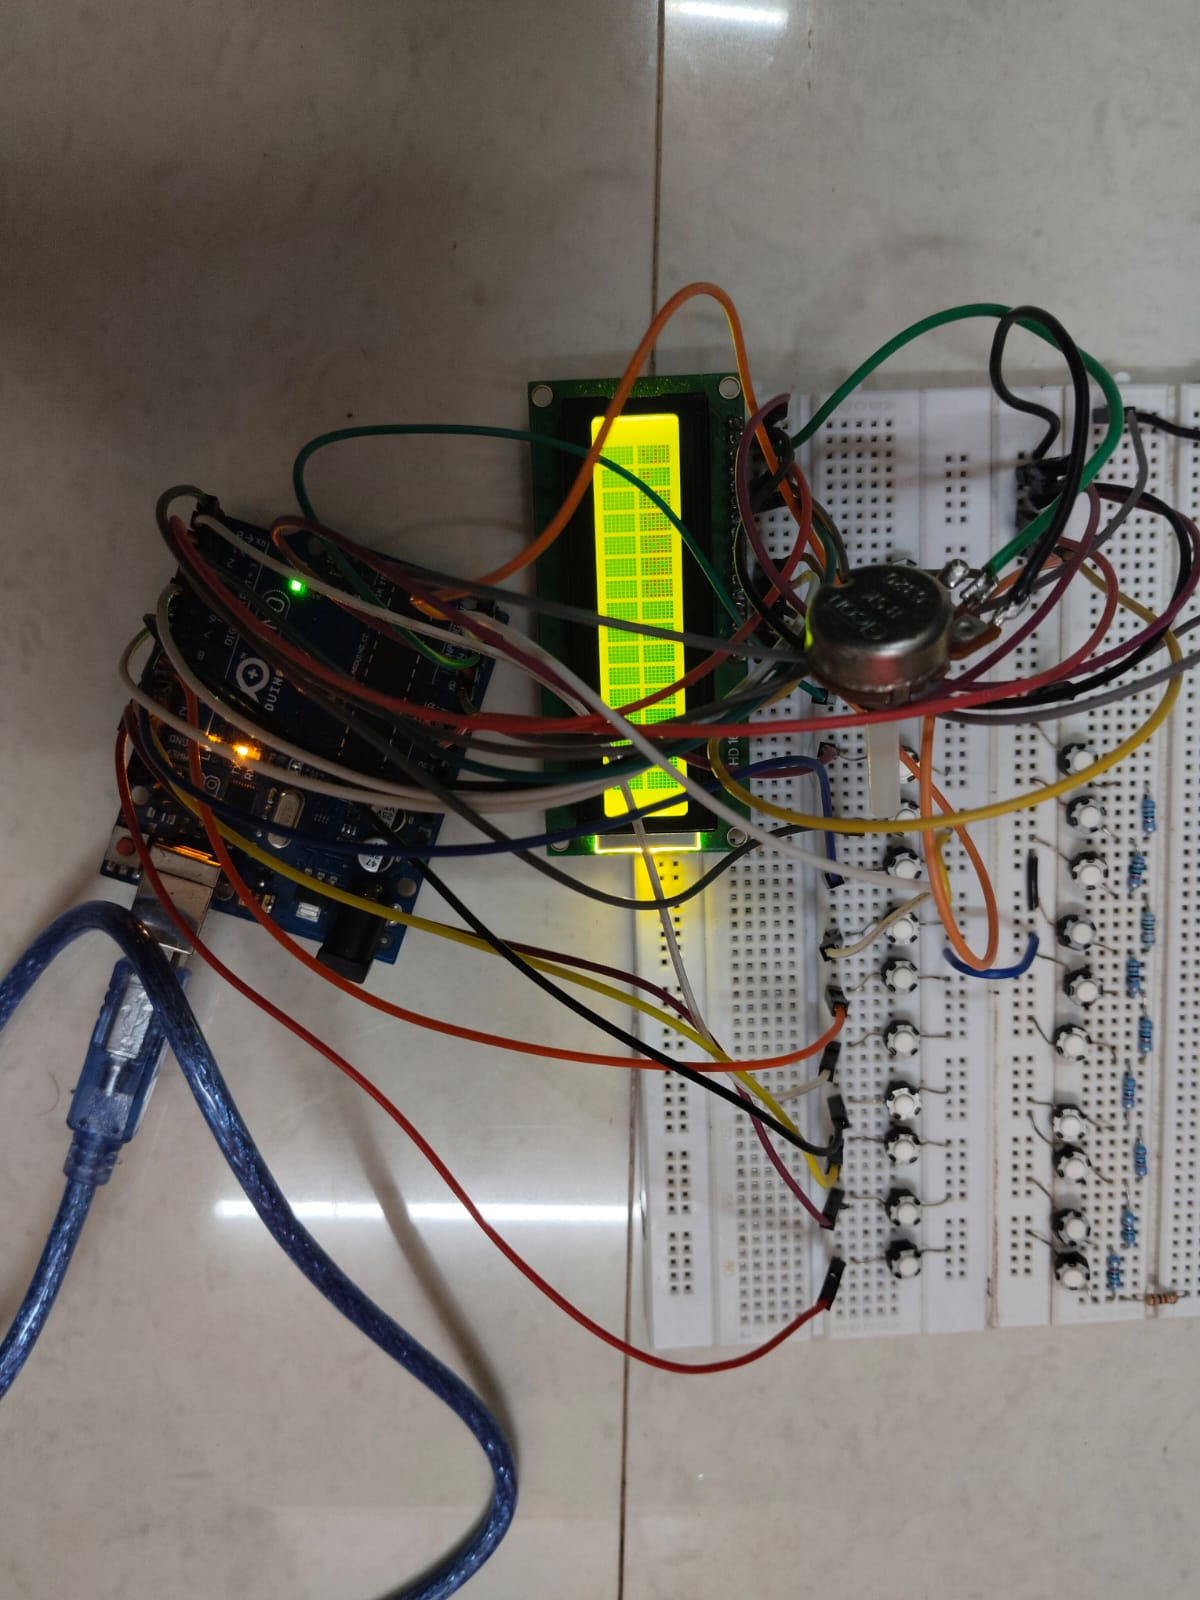
\includegraphics[width=0.5\linewidth]{fig/ckt.jpeg}
    \label{fig:enter-label}
\end{figure}

\section{Analog-to-Digital Conversion (ADC)}

\subsection{ADC Fundamentals}
The ATmega328P's 10-bit ADC converts analog voltages (0-5V) to digital values (0-1023). Key characteristics include:
\begin{itemize}
    \item 10-bit resolution (1024 discrete values)
    \item 9-260$\mu$s conversion time (depending on clock prescaler)
    \item 8 multiplexed input channels (A0-A7)
\end{itemize}

\subsection{Implementation in Calculator}
\begin{itemize}
    \item \textbf{Button:}
    \begin{itemize}
        \item Digit buttons 0-9 connected via voltage divider to A0
        \item Each button produces a unique voltage level (e.g., Button1=0.5V, Button2=1.0V,...,Button9=4.5V)
    \end{itemize}
    
    \item \textbf{Configuration:}
    \begin{itemize}
        \item Reference voltage: AVcc (5V)
        \item Prescaler: 128 (ADC clock = 125kHz)
        \item Channel selection: ADC0 (A0 pin)
    \end{itemize}

    \item \textbf{Reading Process:}
    \begin{itemize}
        \item Single conversion initiated via ADSC bit
        \item \texttt{Conversion complete} flag (ADIF) checked for completion
        \item Result read from ADC/ADCL registers
    \end{itemize}
\end{itemize}

\section{Mathematical implementation}

\subsection{Arithmetic Operations}
\begin{itemize}
    \item Four basic operations with floating-point precision
    \item Operator precedence handling (PEDMAS)
    \item Chained calculation capability 
\end{itemize}

\subsection{Scientific Functions}
\begin{itemize}
    \item Trigonometric functions (sin, cos, tan) with degree/radian modes
    \item Logarithmic functions (base 10 and natural log)
    \item Exponential functions
\end{itemize}


\section{Software Implementation}

The main.c code can be found in the folder named 'codes'.

The following describes the key functions used in the implementation:
\subsection{Core mathematical functions}


\subsubsection{Angle Conversion and Reduction}
\begin{itemize}
\item \texttt{double reduce\_angle(double rad)}:
Reduces any angle to the range $[0, 2\pi)$ by removing full rotations. Essential for trigonometric function stability.

\item \texttt{double deg2rad(double deg)}:
Converts degrees to radians using the formula $rad = deg \times \frac{\pi}{180}$.
\end{itemize}
\subsubsection{Computing $\ln{x}$}
\texttt{double compute\_ln(double x)}:
Calculates natural logarithm using numerical integration of $\int_1^x \frac{1}{t} dt$ with trapezoidal rule.
\subsubsection{Numerical Methods}
\begin{itemize}
\item \texttt{double tangent\_rk4(double radians, double h)}:
Computes tangent using 4th-order Runge-Kutta method by solving the differential equation $\frac{d^2y}{dx^2} = -y$.
\item \texttt{double power(double x, double n)}:
Implements $x^n$ using Euler's method on the differential equation $\frac{dy}{dx} = n \cdot y$.
\end{itemize}

\subsection{Stack Operations}

\subsubsection{Operator Stack}
\begin{itemize}
\item \texttt{void initStack(Stack *s)}: Initializes operator stack.
\item \texttt{void push(Stack *s, const char* val)}: Pushes operator onto stack.
\item \texttt{const char* peek(Stack *s)}: Views top element without removal.
\end{itemize}

\subsubsection{Number Stack}
\begin{itemize}
\item \texttt{void initNumStack(NumStack *s)}: Initializes operand stack.
\item \texttt{void pushNum(NumStack *s, float val)}: Pushes number onto stack.
\item \texttt{float popNum(NumStack *s)}: Removes and returns top number.
\end{itemize}

\subsection{Expression Processing}

\subsubsection{Infix to Postfix Conversion}
\begin{itemize}
\item \texttt{void infixToPostfix(const char* infix, char* postfix)}:
Converts standard mathematical notation to Reverse Polish Notation using Dijkstra's shunting-yard algorithm. Handles:
\begin{itemize}
\item Parentheses grouping
\item Operator precedence (PEMDAS)
\item Special functions (trig, log)
\end{itemize}
\end{itemize}

\subsubsection{Postfix Evaluation}
\begin{itemize}
\item \texttt{float evaluatePostfix(const char* postfix)}:
Evaluates RPN expressions using a number stack. Supports:
\begin{itemize}
\item Basic arithmetic ($+,-,\times,\div$)
\item Exponents ($x^y$)
\item Trigonometric functions ($\sin,\cos,\tan$)
\item Logarithmic functions ($\ln,\log_{10}$)
\end{itemize}
\end{itemize}

\subsection{Utility Functions}

\subsubsection{Fraction Conversion}
\begin{itemize}
\item \texttt{void decimal\_to\_fraction(double decimal, int *numerator, int *denominator)}:
Converts floating-point numbers to simplified fractions using continued fractions approximation with tolerance $10^{-6}$.
\end{itemize}

\subsubsection{LCD Interface}
\begin{itemize}
\item \texttt{void lcd\_init(void)}:
Initializes 16x2 LCD in 4-bit mode with proper timing delays.

\item \texttt{void lcd\_print(const char* str)}:
Outputs strings with character-by-character timing control.

\item \texttt{void lcd\_set\_cursor(uint8\_t col, uint8\_t row)}:
Positions cursor using DDRAM address mapping.
\end{itemize}


\subsubsection{ADC Handling}
\begin{itemize}
\item \texttt{uint16\_t adc\_read(uint8\_t channel)}:
Reads analog inputs with:
\begin{itemize}
\item 3-sample moving average
\item Hysteresis filtering ($\pm25$ counts)
\item Channel auto-selection
\end{itemize}
\end{itemize}

\subsection{Main Program Flow}
The calculator implements an event loop that:
\begin{enumerate}
\item Scans buttons via ADC and digital inputs
\item Processes keypresses with debouncing
\item Maintains input buffer (16-character limit)
\item Converts and evaluates expressions on ENTER
\item Displays results in decimal or fraction form
\end{enumerate}

\section{Results and Discussion}

The calculator worked correctly when pressing buttons and displayed the right numbers. All calculations were accurate during testing. The system ran smoothly without any problems for continuous operation and implemented PEDMAS effectively.\\
Example:(Implementing PEDMAS)\\

\begin{figure}[H]
        \centering
        \begin{minipage}{0.45\linewidth}
        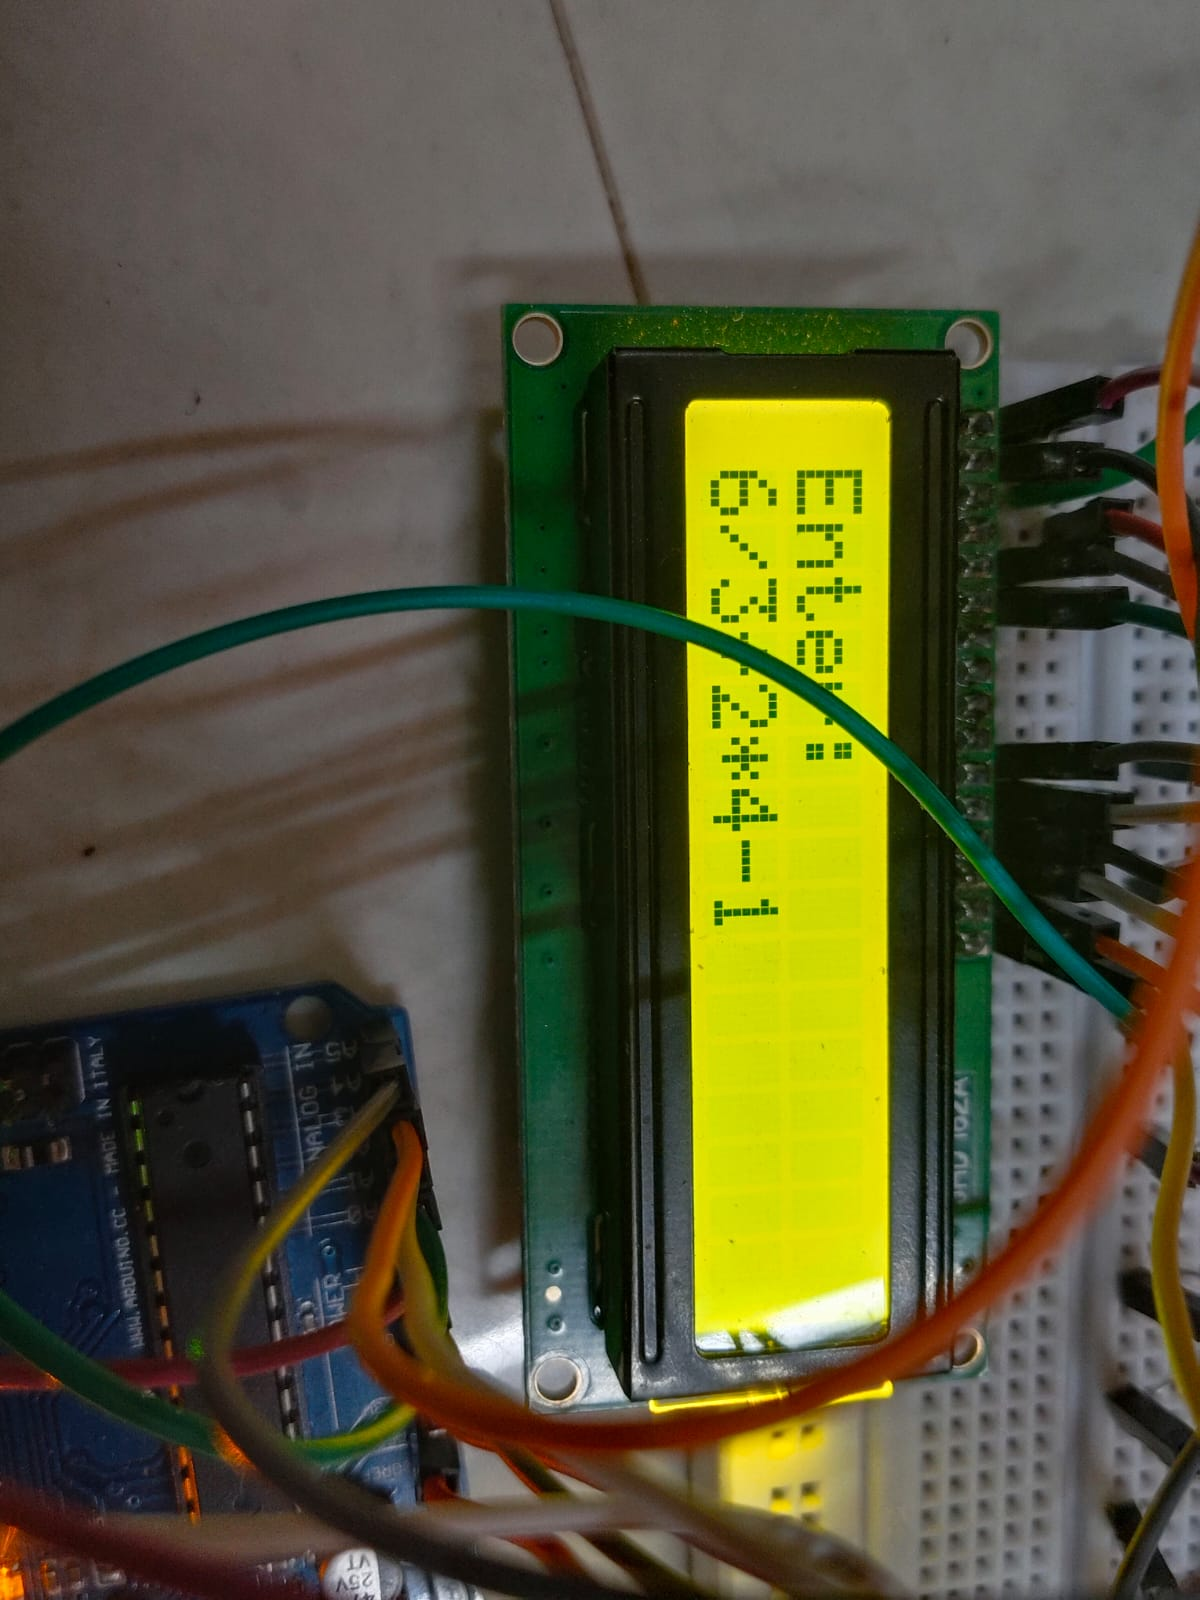
\includegraphics[width=1.0\linewidth]{fig/dmas.jpeg}
        \label{fig:enter-label}
        \end{minipage}
        \hfill
        \begin{minipage}{0.45\linewidth}
        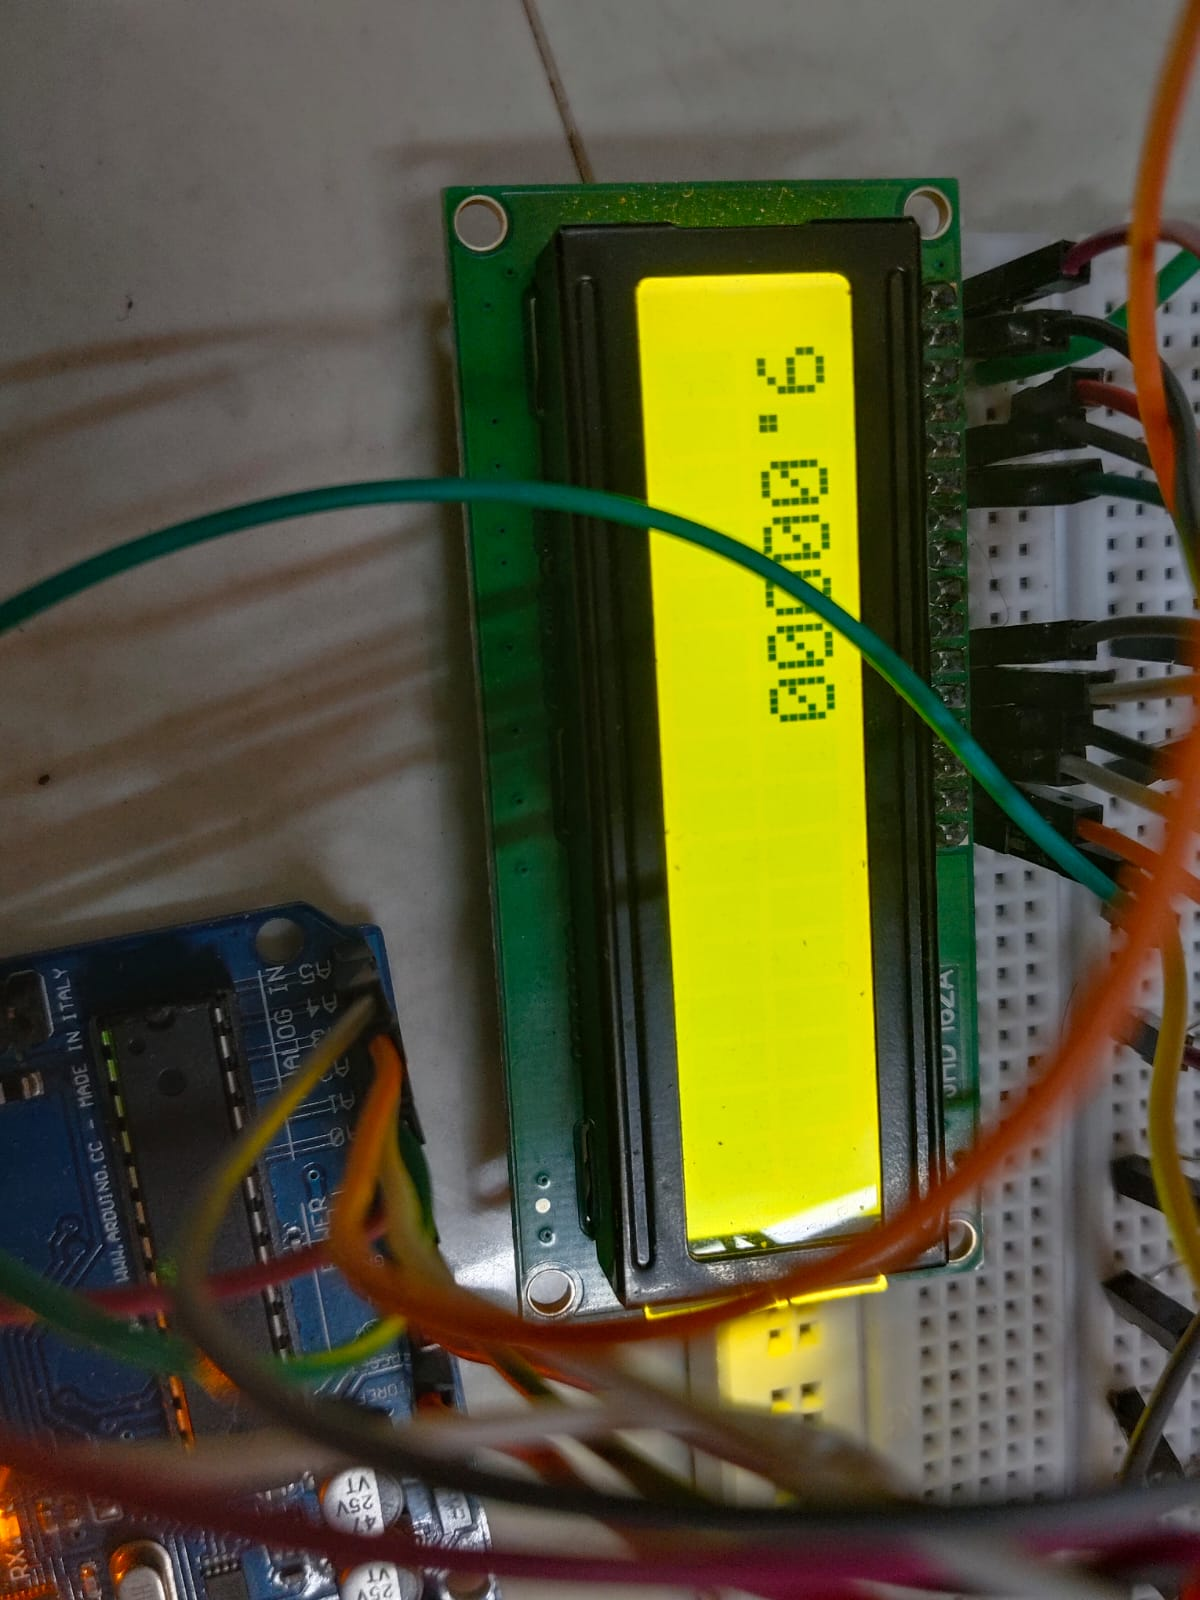
\includegraphics[width=1.0\linewidth]{fig/dmas0.jpeg}
        \label{fig:enter-label}
        \end{minipage}
\end{figure}

\section{Conclusion}
This project successfully demonstrates the implementation of a scientific calculator using embedded systems principles. The design makes efficient use of available microcontroller resources while providing comprehensive mathematical functionality. 
\end{document}
